%%%%%%%%%%%%%%%%%%%%%%%%%%%%%%%%%%%%%%%%%%%%%%%%%%%%%%%%%%%
%                                                         %
%       This is documentation for the IPK project.        %
%                                                         %
%%%%%%%%%%%%%%%%%%%%%%%%%%%%%%%%%%%%%%%%%%%%%%%%%%%%%%%%%%%


%------------------------------------------------%
%	    CONFIGURATION + IMPORTED PACKAGES        %
%------------------------------------------------%
\documentclass[10pt,a4paper,titlepage]{article}
\usepackage[english]{babel}
\usepackage[utf8]{inputenc}
\usepackage[margin=100pt]{geometry}


\usepackage{graphicx}   % Import pictures
\usepackage{ragged2e}   % fullfill paragraphs
\usepackage{multicol}
\usepackage{lscape}
\usepackage{xcolor}
\usepackage{listings}
\usepackage{courier}

\definecolor{mGreen}{rgb}{0,0.6,0}
\definecolor{mGray}{rgb}{0.5,0.5,0.5}
\definecolor{mPurple}{rgb}{0.58,0,0.82}
\definecolor{backgroundColour}{rgb}{0.95,0.95,0.92}

\lstdefinestyle{CStyle}{
    commentstyle=\color{mGreen},
    keywordstyle=\color{magenta},
    numberstyle=\tiny\color{mGray},
    stringstyle=\color{mPurple},
    basicstyle=\scriptsize\ttfamily,%\tiny\ttfamily,
    breakatwhitespace=false,
    columns=fullflexible,
    breaklines=true,
    captionpos=b,
    keepspaces=true,
    language=C
}

\newenvironment{changemargin}[2]{%
\begin{list}{}{%
\setlength{\topsep}{0pt}%
\setlength{\leftmargin}{#1}%
\setlength{\rightmargin}{#2}%
\setlength{\listparindent}{\parindent}%
\setlength{\itemindent}{\parindent}%
\setlength{\parsep}{\parskip}%
}%
\item[]}{\end{list}}

%\usepackage{biblatex}
\usepackage[backend=biber]{biblatex}
\addbibresource{dokumentace.bib}

\begin{document}
%-----------------------------------------%
%	            TITLE PAGE                %
%-----------------------------------------%
\begin{titlepage}

\begin{center}
% Headings
\textsc{\LARGE Brno University of technology}\\[0.5cm]
\textsc{\large Faculty of Information Technology}\\[8cm]

% Title - lines
{ \huge \bfseries IPK project 1}\\[0.3cm]
{ \Large \bfseries documentation}\\[0.5cm]
{ \bfseries Martin Benes}\\

\end{center}

\end{titlepage}
\newpage

%-----------------------------------------%
%	              DOCUMENT                  %
%-----------------------------------------%

\pagenumbering{gobble}

\section*{IPK project documentation}
The task was to create an client-server application in C/C++, that communicates
using BSD sockets and transfers files.

We ought to design our own protocol, that we use for the communication, and
describe it in documentation in detail.

\subsection*{Protocol description}
I started with an analysis of BSD socket interface. Since it is C library,
the classical C-style approach appeared to me more suitable in this case,
considering the project size. The~protocol is built on TCP protocol,
because it needs reliable transmission.

{\it TCP creates a {\bf reliable data transfer service} on top of IP's unreliable
best-effort service. TCP's reliable data transfer service ensures that the
data stream that process reads out of its TCP receive buffer is uncorrupted,
without gaps, without duplication, and in sequence; that is, the byte stream
is exactly the same byte stream that was sent by the end system on the other
side of the connection.} \cite[p.~238]{computernetworking}.

\begin{multicols}{2}
The protocol was described on two levels of abstraction, simplifying its
relative complexity. The lower one specifies the sending of single
buffer. Due to the BSD sockets specification, where the receiver
does not know the size of data he acquires, the protocol sends a packet
(of {\it sizeof(size\_t)}) with the~size of data that will follow,
and the data itself afterwards.

So when the receiver reads the data, he already knows their size.

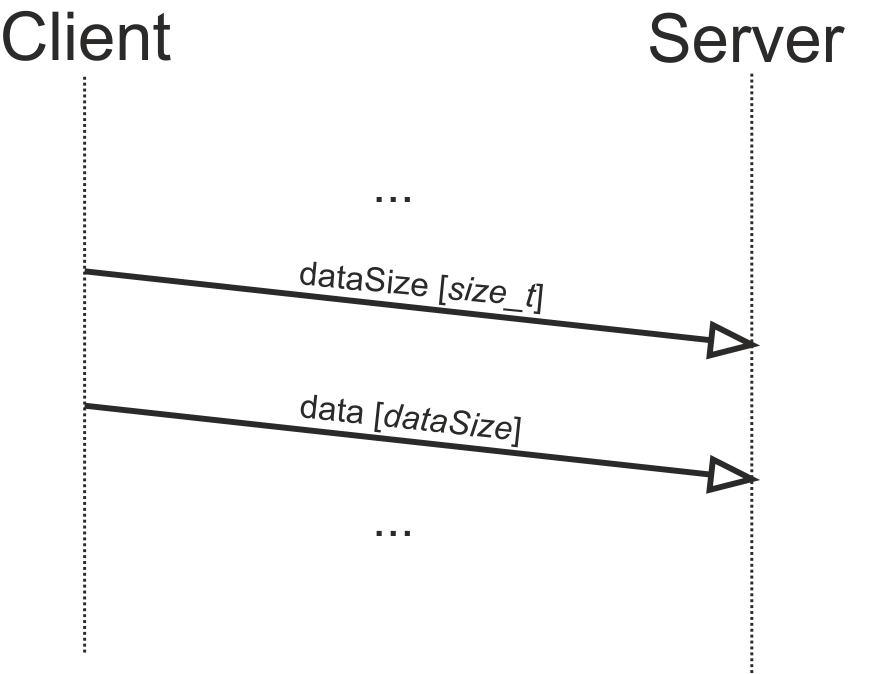
\includegraphics[width=0.45\textwidth]{send_data.png}
\end{multicols}


\begin{multicols}{2}
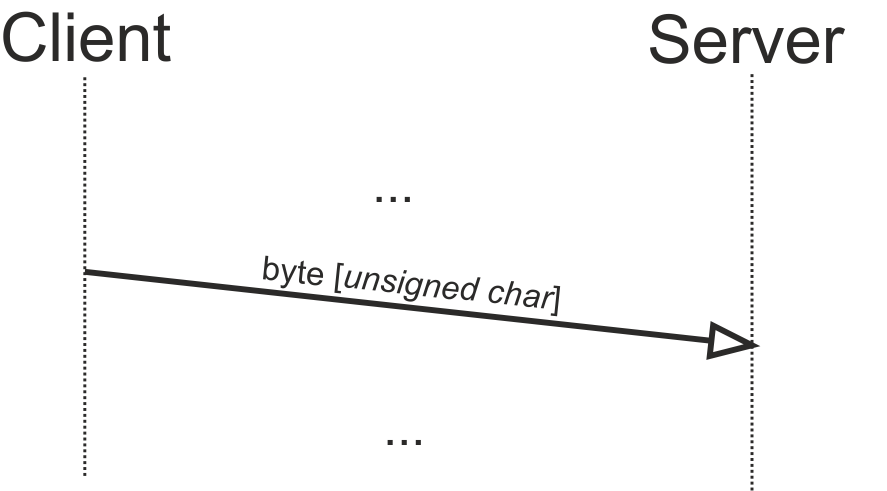
\includegraphics[width=0.4\textwidth]{send_byte.png}

The protocol may send a single byte too. It is used to send an indication
to the opposite side, such as errors etc., the~client sends the mode
(read/write), or server announces if the reading of file succeeds.

In this case, the sent data are fixed-sized ({\it unsigned~char}),
so it does not have to do the same routine as the above mentioned.
\end{multicols}


The higher abstraction layer (the program itself) uses the services of the
lower. The~server is listening on the port and the client is connecting to the
server with explicitly given address and port. The mode of usage (read/write)
is also given.

During the implementation, I have encountered several problems. The most
significant one pushed me to the the segmentation of the message on my own.
When the data are to be sent, they are read as segments ({\it by 1024~B})
and sent like that, preceeded by total size, as was mentioned above.
The opposite side receives them and it substracts the total data received.
When the last buffer receives, the receiver knows exactly, how big is the
part that contains valid data.

This makes the problem a bit more complicated, but it prevents the problem
with too big files, that would not fit into RAM.

Every segment sent is followed with ACK packet, that confirms its arrival.
It slows the process a lot, but it is worth it, anyway the lost packets would
get lost.

\begin{multicols}{2}
The read is initiated, when argument {\it -r} is given, following with a
{\it path}. The first to send as a client is a byte 0xFF, that means the reading
mode is selected.

The second thing to send is a single {\it filename}. Afterwards, the {\it file}
itself is expected to receive from the server.

Then the data are sent, the described procedures are used here.

The client then writes the arriving data into the file of the name, here into
the full path, that was given.

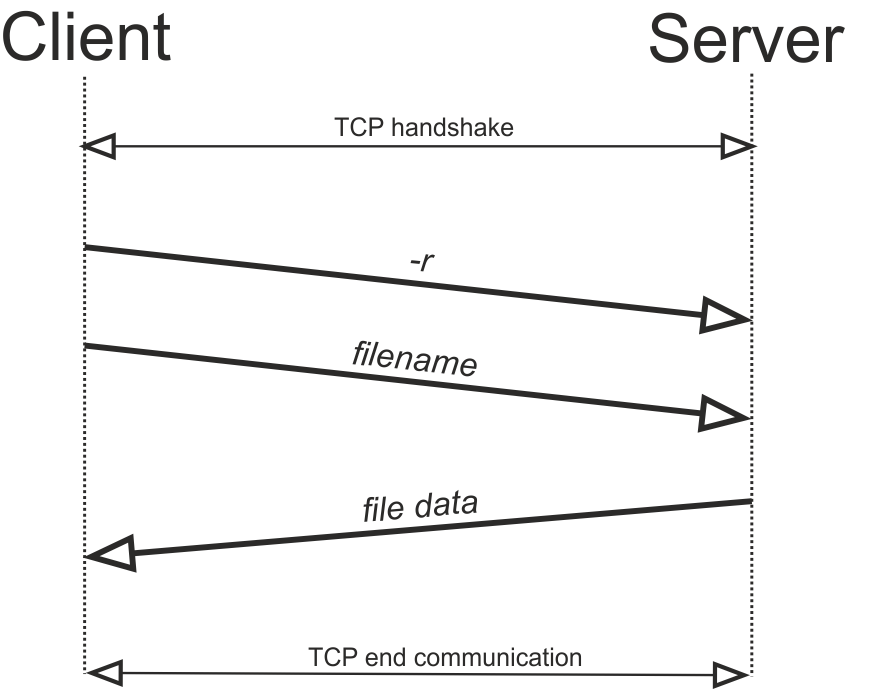
\includegraphics[width=0.5\textwidth]{read.png}
\end{multicols}


\begin{multicols}{2}

The write is similar as read with slight differences, it is initialized
with a given argument {\it -w} and the {\it path} afterwards. The first byte
is 0x0F, indicating the write mode.

Then the client sends {\it the name of the file} (without the path), on the
server, it will be located in the working directory.

The client follows with sending {\it the file data}. Again, it is done
with the mentioned method.

The server then writes the received data to the file.

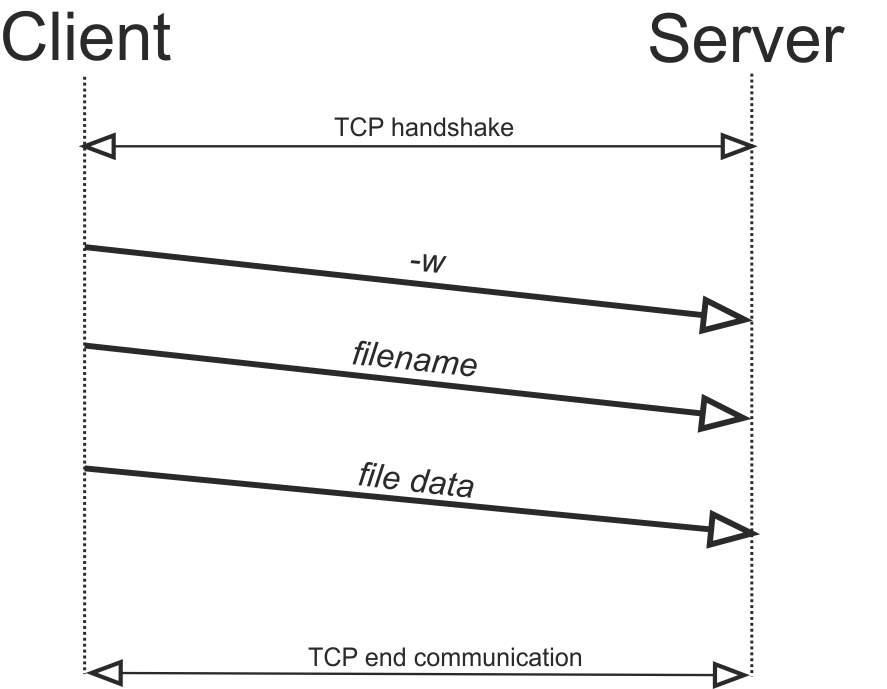
\includegraphics[width=0.5\textwidth]{write.png}
\end{multicols}

\subsection*{Client state diagram}

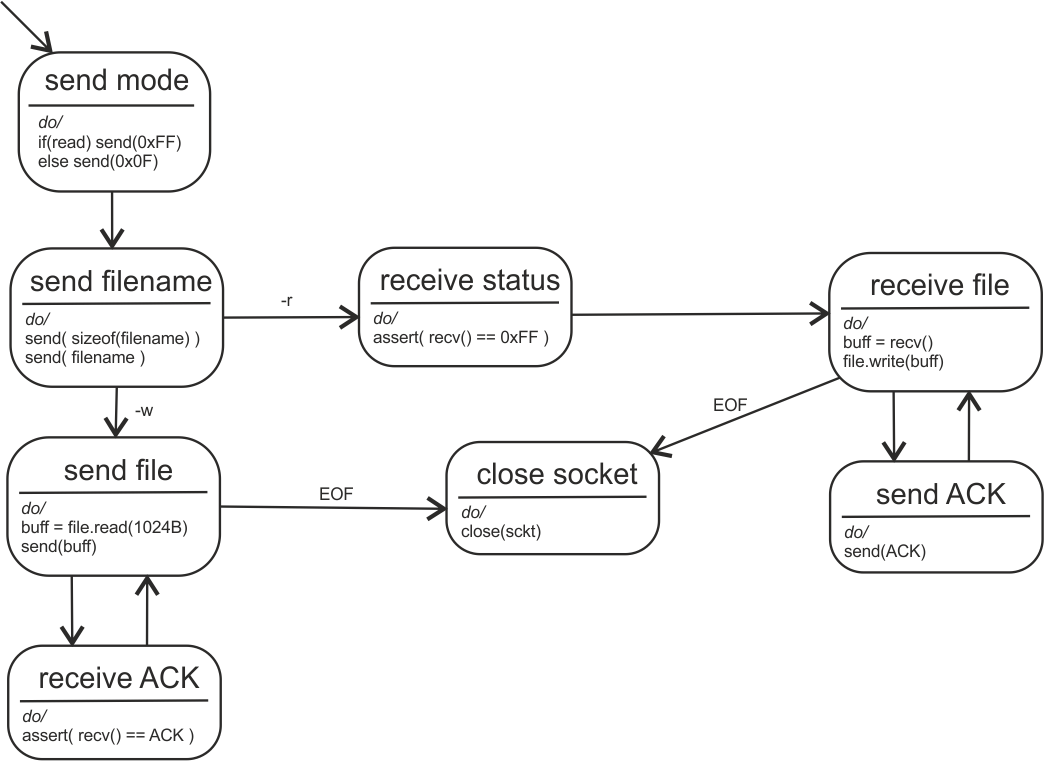
\includegraphics[width=0.9\textwidth]{state_client.png}

\subsection*{Server state diagram}

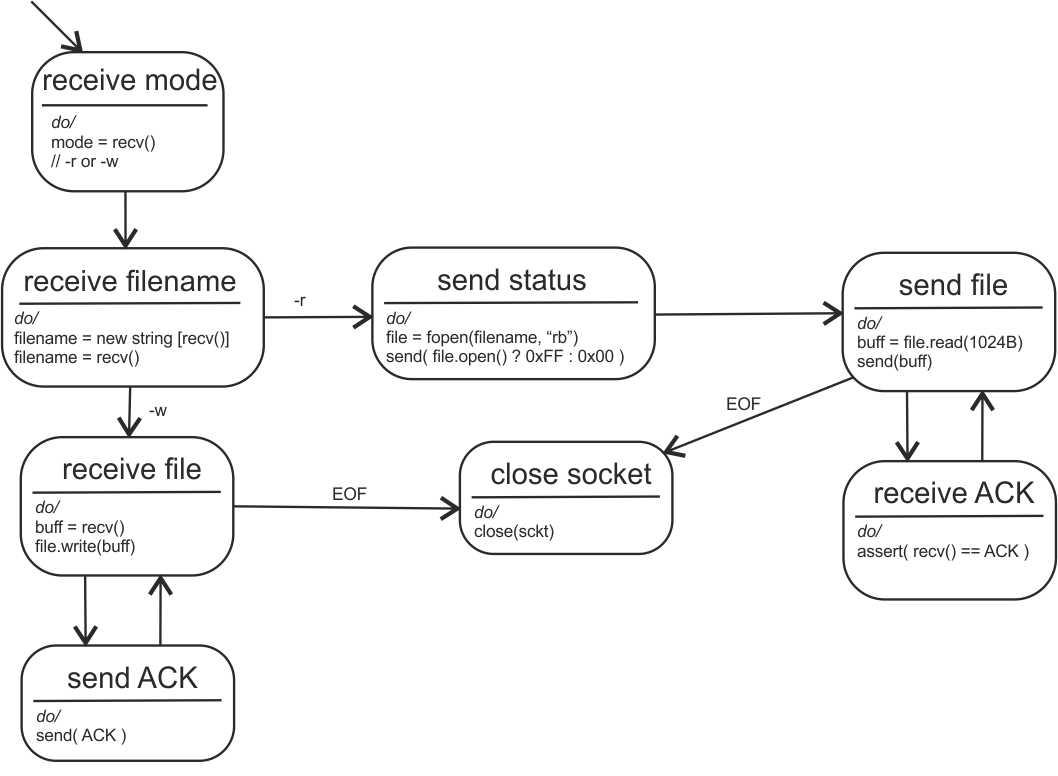
\includegraphics[width=0.9\textwidth]{state_server.png}

\subsection*{Implementation}

There are two programs, {\it ipk-server} and {\it ipk-client}, each has its
own module, {\it server.cpp} and {\it client.cpp}. They contain implementation
of the whole protocol, as described above.

The server is concurrent, using {\it fork()} call and utilities from
{\it signal.h} standard C library, which means it can operate with multiple
clients at one time.

There is also a common module used by both of the programs, {\it defs.h}.
It includes debug constants, common functions and a {\it Config} class,
which is used to process arguments, to check if they are valid for the program
it is used in and to hold the configuration of the program.



\begin{multicols}{2}

\begin{lstlisting}[style=CStyle]
  /* ----- client.cpp ----- */
  // send mode (read/write)
  unsigned char mode = conf.read()?0xFF:0x0F;
  send(sckt, &mode, sizeof(char), 0);
  if(conf.read())
    PerformRead(sckt);  // read
  else
    PerformWrite(sckt); // write
\end{lstlisting}

\begin{lstlisting}[style=CStyle]
  /* ----- server.cpp ----- */
  // receive mode (read/write)
  unsigned char mode;
  recv(comm, &mode, sizeof(mode), 0);
  if( mode == 0xFF )
    PerformRead(comm);  // read
  else
    PerformWrite(comm); // write
  // no return here
\end{lstlisting}

\end{multicols}
\printbibliography

\end{document}
